\chapter{Web Application Implementation}%
This chapter describes the web application which was created for this thesis. The main purpose of the application was to present discussed algorithms
and the results collected during this study. One of the main assumptions of this application was to make it available to others. The purpose was to
easily share this application, therefore it was written as a web frontend application. The application and its repository are publicly available at~\cite{26, 27}.
\section{Technologies Used}
The following sections describe the technological stack used while building the application. It also provides a guide to the user interface. The application 
was supposed to have a modern look and feel, and be interactive and responsive for its users. The source code \cite{27} provides a full implementation of all algorithms,
views and scripts needed to correctly run this application. There is no database connection provided because there was no logical reason to create a user
authentication or save the results in a database. Each user can export data generated with this application to a PDF file. The project was developed using a free
IDE Visual Studio Code.
\subsection{HTML, CSS and Bootstrap}
The main task of this application was to create a presentation layer. Each application view was written in HTML files. HTML is the markup language which
gives structure and meaning to web content and is a cornerstone of each web page or application. The second layer of the standard web stack is styling with CSS.\\
CSS is a language of style rules which apply styling to structured HTML content. As the design of the UI consists of many different components, uniform
bootstrap styling was used. Bootstrap~\cite{28} is a free, open-source front-end development framework for the creation of websites and web apps. It utilizes a prebuilt
grid system and components. It also provides dozens of CSS variables. Bootstrap was chosen also because JavaScript in Bootstrap is HTML-first. The implemented 
application does not contain any convoluted or many dynamic features so it was developed using only JavaScript. Therefore there was no reason to overcomplicate it
with JQuery which is a popular JavaScript library which makes HTML document traversal, manipulation and event handling much simpler with an easy-to-use multi-browser API.%
\subsection{JavaScript}
The secondary part of this thesis was to implement and compare algorithms. As the web application was arbitrarily chosen to be developed, hence JavaScript was the 
clear choice as it is third, after HTML and CSS, key layer component of modern web development. All maze-related algorithms were implemented in JavaScript.
It may be noticed that from the performance perspective JavaScript should not be the apparent choice. However, the objective of this study was not to maximize
the performance, a more low-level language would be better for such a case. JavaScript is a lightweight interpreted programming language. 
It combines two important features. On the one hand, it allows building object-oriented logic for the implemented algorithms due to some common programming
features. On the other hand, it provides tools for dynamically changing the content of web applications \cite{29}. Furthermore, the most useful functionality built on top
of the client side is a Browser's API, an Application Programming Interface which can expose data from the surrounding computer environment. For this work, it was necessary to use two browser APIs, i.e. DOM and canvas. DOM is a Document Object Model that allows dynamically manipulate with HTML and CSS.
Canvas is for creating 2D graphics which was used in the maze generation component to visualise the generated mazes and their solution. 
\subsection{Charts.js}
Chart.js~\cite{30} is a free, open-source JavaScript library used for data visualisation. It allows to easy create different types of dynamic charts. Chart.js renders in 
HTML5 canvas component. It is a well-known library, which is easy to use. In the application, two scatter plots are implemented with three category classes 
for each solver. It also provides an animated look for generated charts out of the box.
\subsection{GitHub Pages}
The created app is publicly available through hosting by GitHub Pages\cite{28}. GitHub Pages is a static site hosting service for client-side-only applications, it does not support
server-side languages. It builds a web page directly from the GitHub Repository of the Project. Service takes HTML, CSS and JavaScript, and runs the files through
the Jekyll building process and publishes a website on the github.io domain or custom domain for free. Jekyll is a static site generator with built-in support for 
GitHub Pages and a simplified build process. Jekyll takes Markdown and HTML files and creates a completely static website. After each push to the repository a GitHub
Action is initialised. GitHub Actions is a continuous integration and continuous delivery (CI/CD) platform that allows automating the build, test, and deployment
pipeline. However, published GitHub Pages have some restrictions: sites may be no larger than 1 GB, and have a soft bandwidth limit of 100 GB per month. For security purposes, 
when a GitHub Pages site is visited, the visitor's IP address is logged and stored by GitHub.\\  
\section{User Interface}
The user interface was created using the components included in the Bootstrap and Charts.js libraries, described in subsections 6.1.2 and 6.1.4.
The home page is the most important view of the application. It is a dashboard of many components. It contains a form for a maze data generator, data visualisation
on canvas components, a table for collected data and a form for choosing the solver.\\
\subsection{UI template}
In this section, all key features of the user interface are described. The starting page of the application is presented in Figure 6.1. It is a blank template which can be
filled with data generated by a user utilising the user interface and implemented algorithms. The template is divided into 5 different parts to provide the optimum
user experience. The application allows the user to generate different types of mazes. Besides three base algorithms, the user can add cycles or directions.
After maze creation, the user can follow the path and parameters of solvers. All data is visualised in two plots, and all data is collected in a table which may be extracted to
the pdf file. The user interface is responsive so it can be also used on mobile devices.
\begin{figure}[!h]
    \centering
    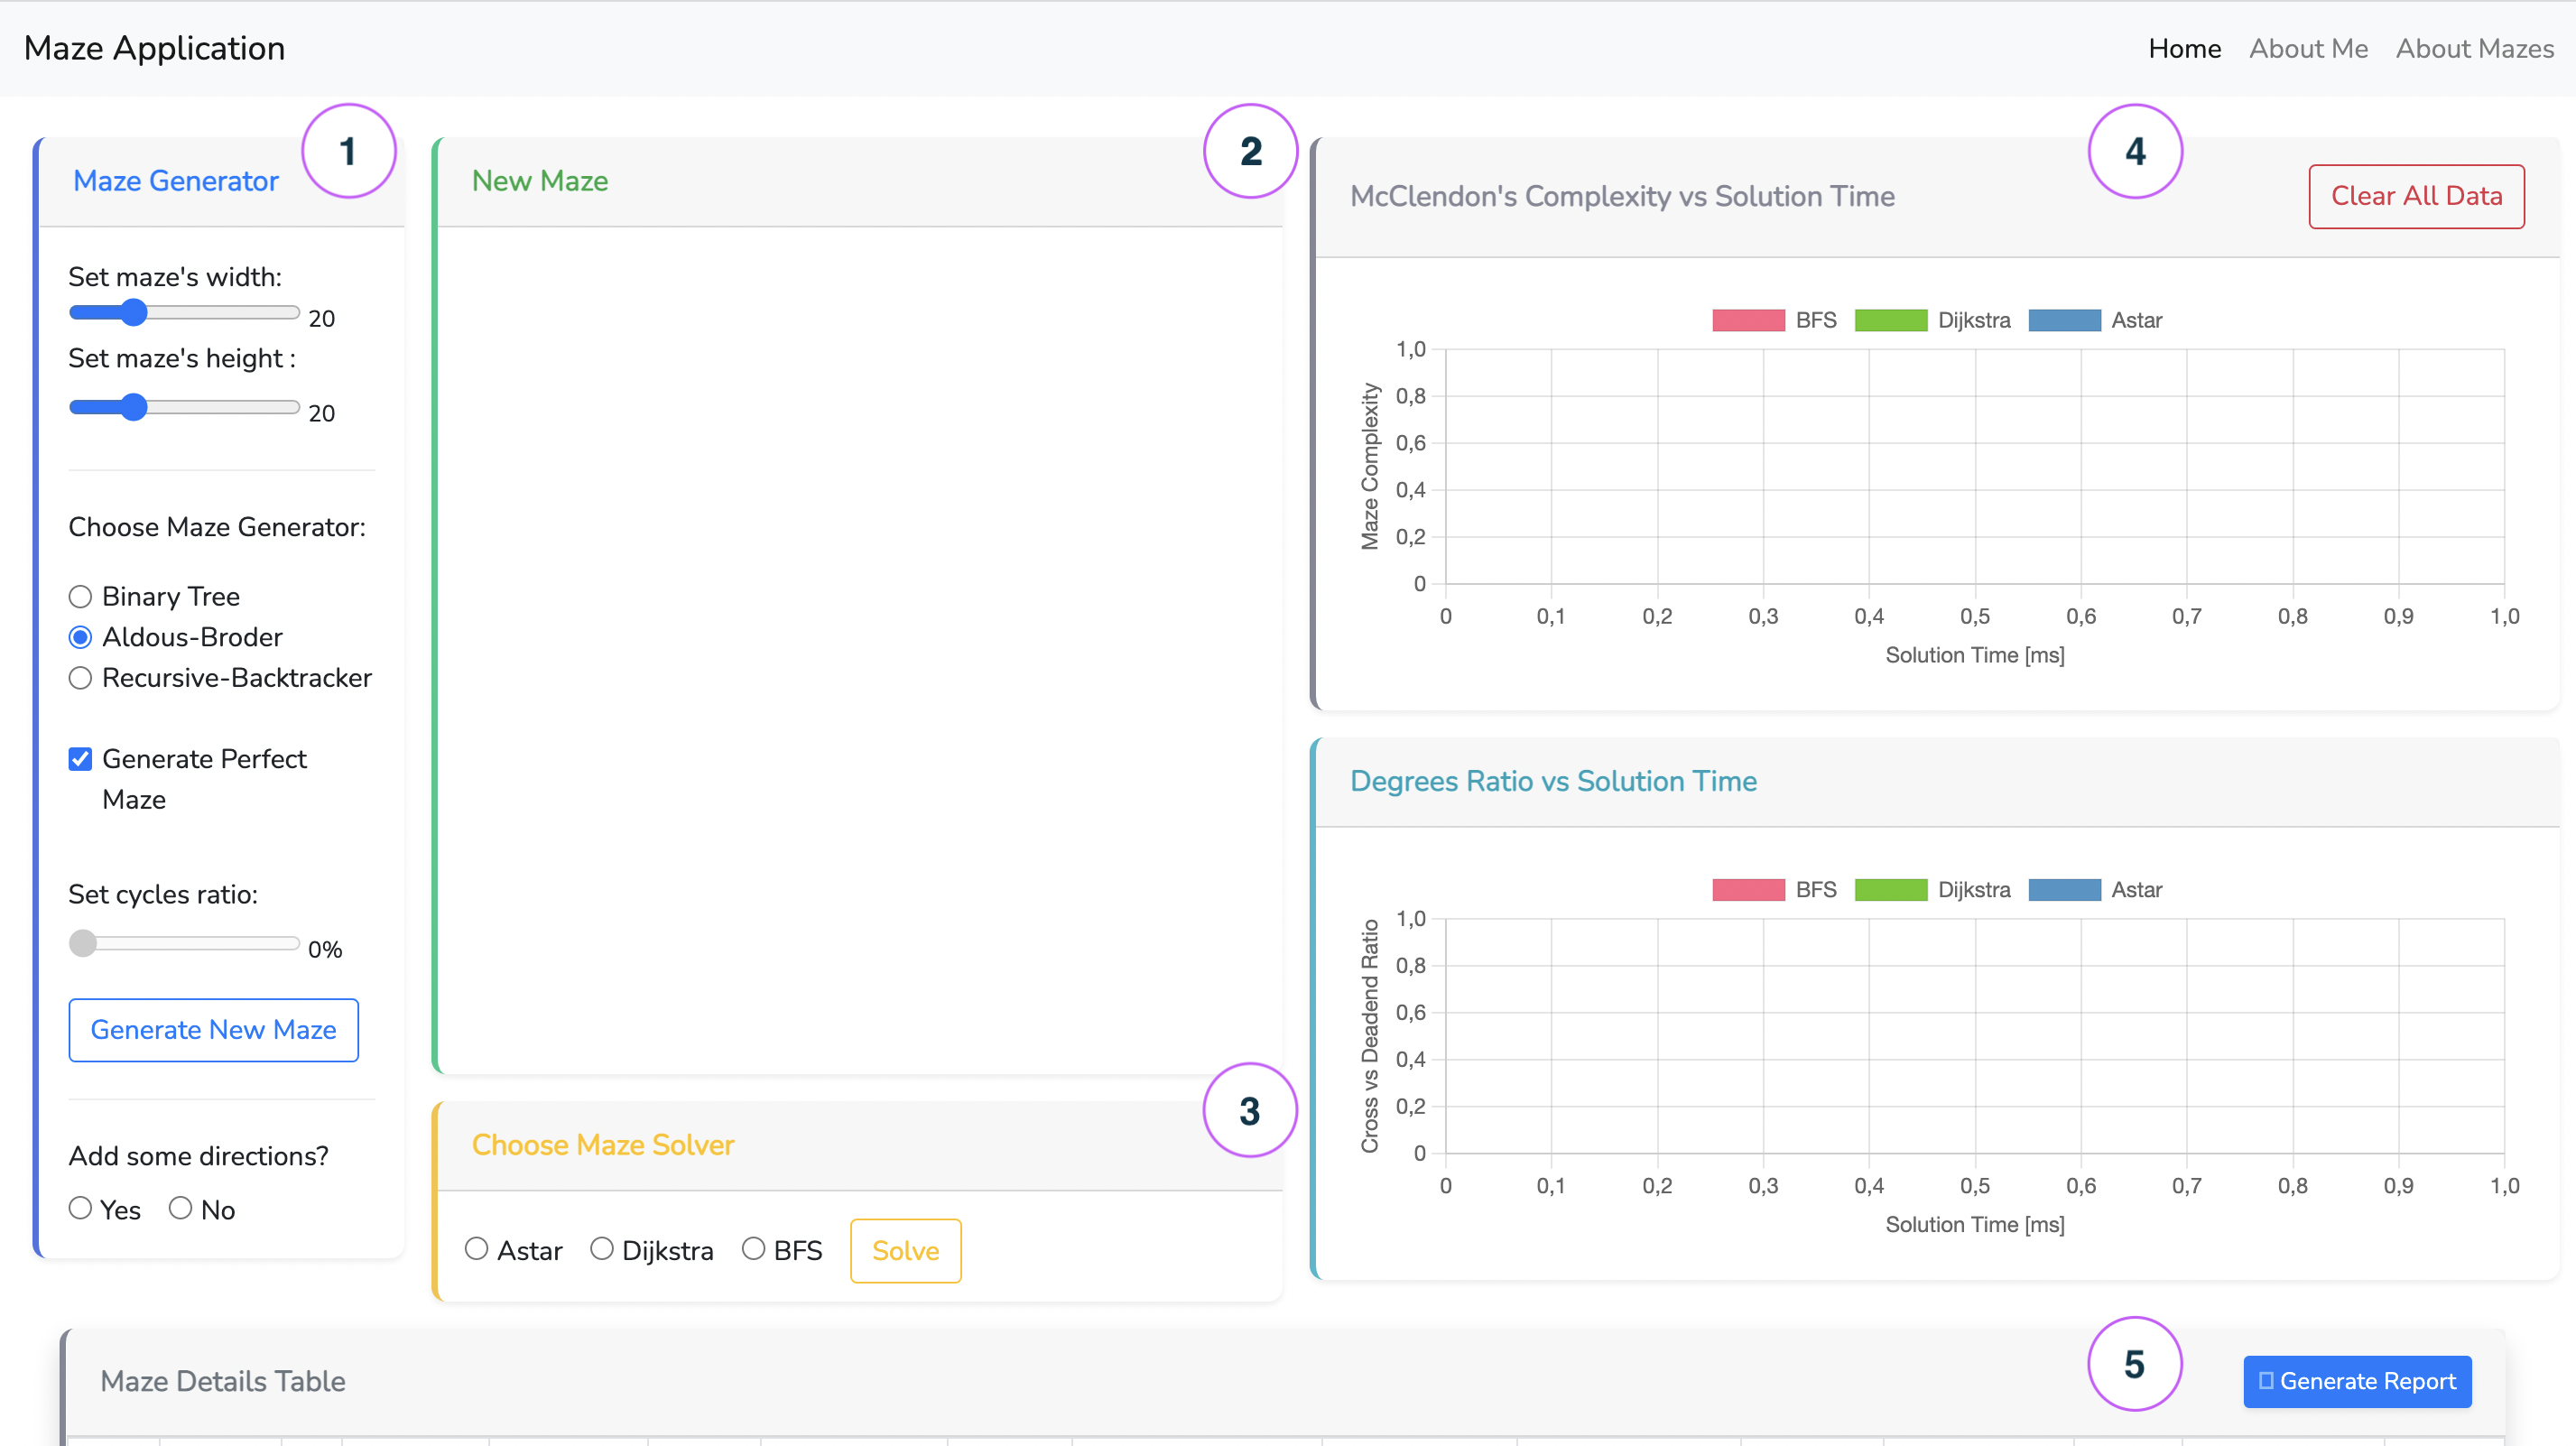
\includegraphics[width=0.9\linewidth]{templateView}
    \caption{Main view of the most important part of the application. The figure presents an empty template before any user actions. All main parts are 
    marked by a number in a pink circle. Maze Generator (1), Maze canvas (2), Solver Section (3), Charts Section (4), Data Table (5).\\ Source: created by the author.}
    \end{figure}
\newpage
\textbf{$-$ Maze Generator}\\
This section is a form which allows users to set all parameters before generating a maze. The form component is presented in Figure 6.2. There are a few options to
choose. Users can set the rectangular maze size by setting the range. There are three implemented generating algorithms to choose from. Users can also check the
Perfect Maze checkbox to generate a perfect maze, or can add some cycles to the maze, by setting the ratio range input. After clicking the Generate Button, the maze
is populated into the canvas component.\\
\begin{figure}[!h]
    \centering
    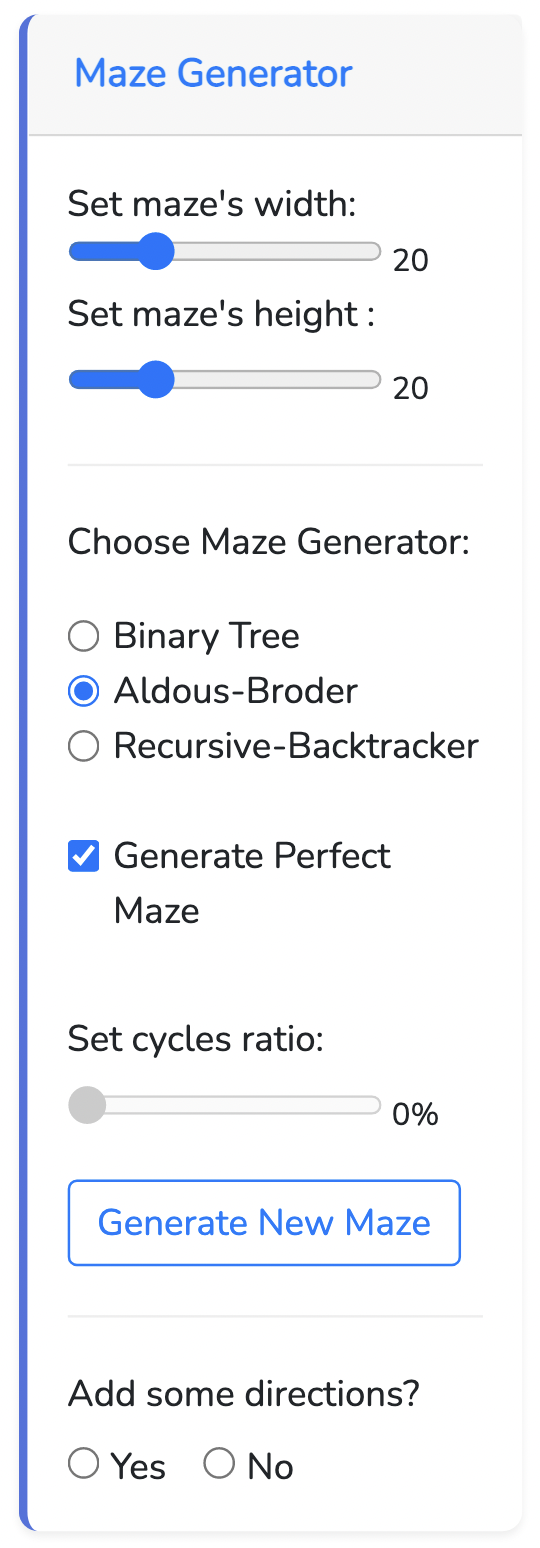
\includegraphics[scale = 0.4]{mazeGenerator}
    \caption{Maze Generator Form.\\Source: created by the author.}
    \end{figure}
\newline   
\textbf{$-$Maze Canvas}\\
When the maze is ready on canvas, the user can select, using radio buttons, if they want to add some directed edges to the maze before solving. If yes, the user can do it 
by clicking cells in canvas eg. in Figure 6.3. The direction implemented is, so the flow for cells marked green can happen only in one, north direction.\\
\begin{figure}[!h]
    \centering
    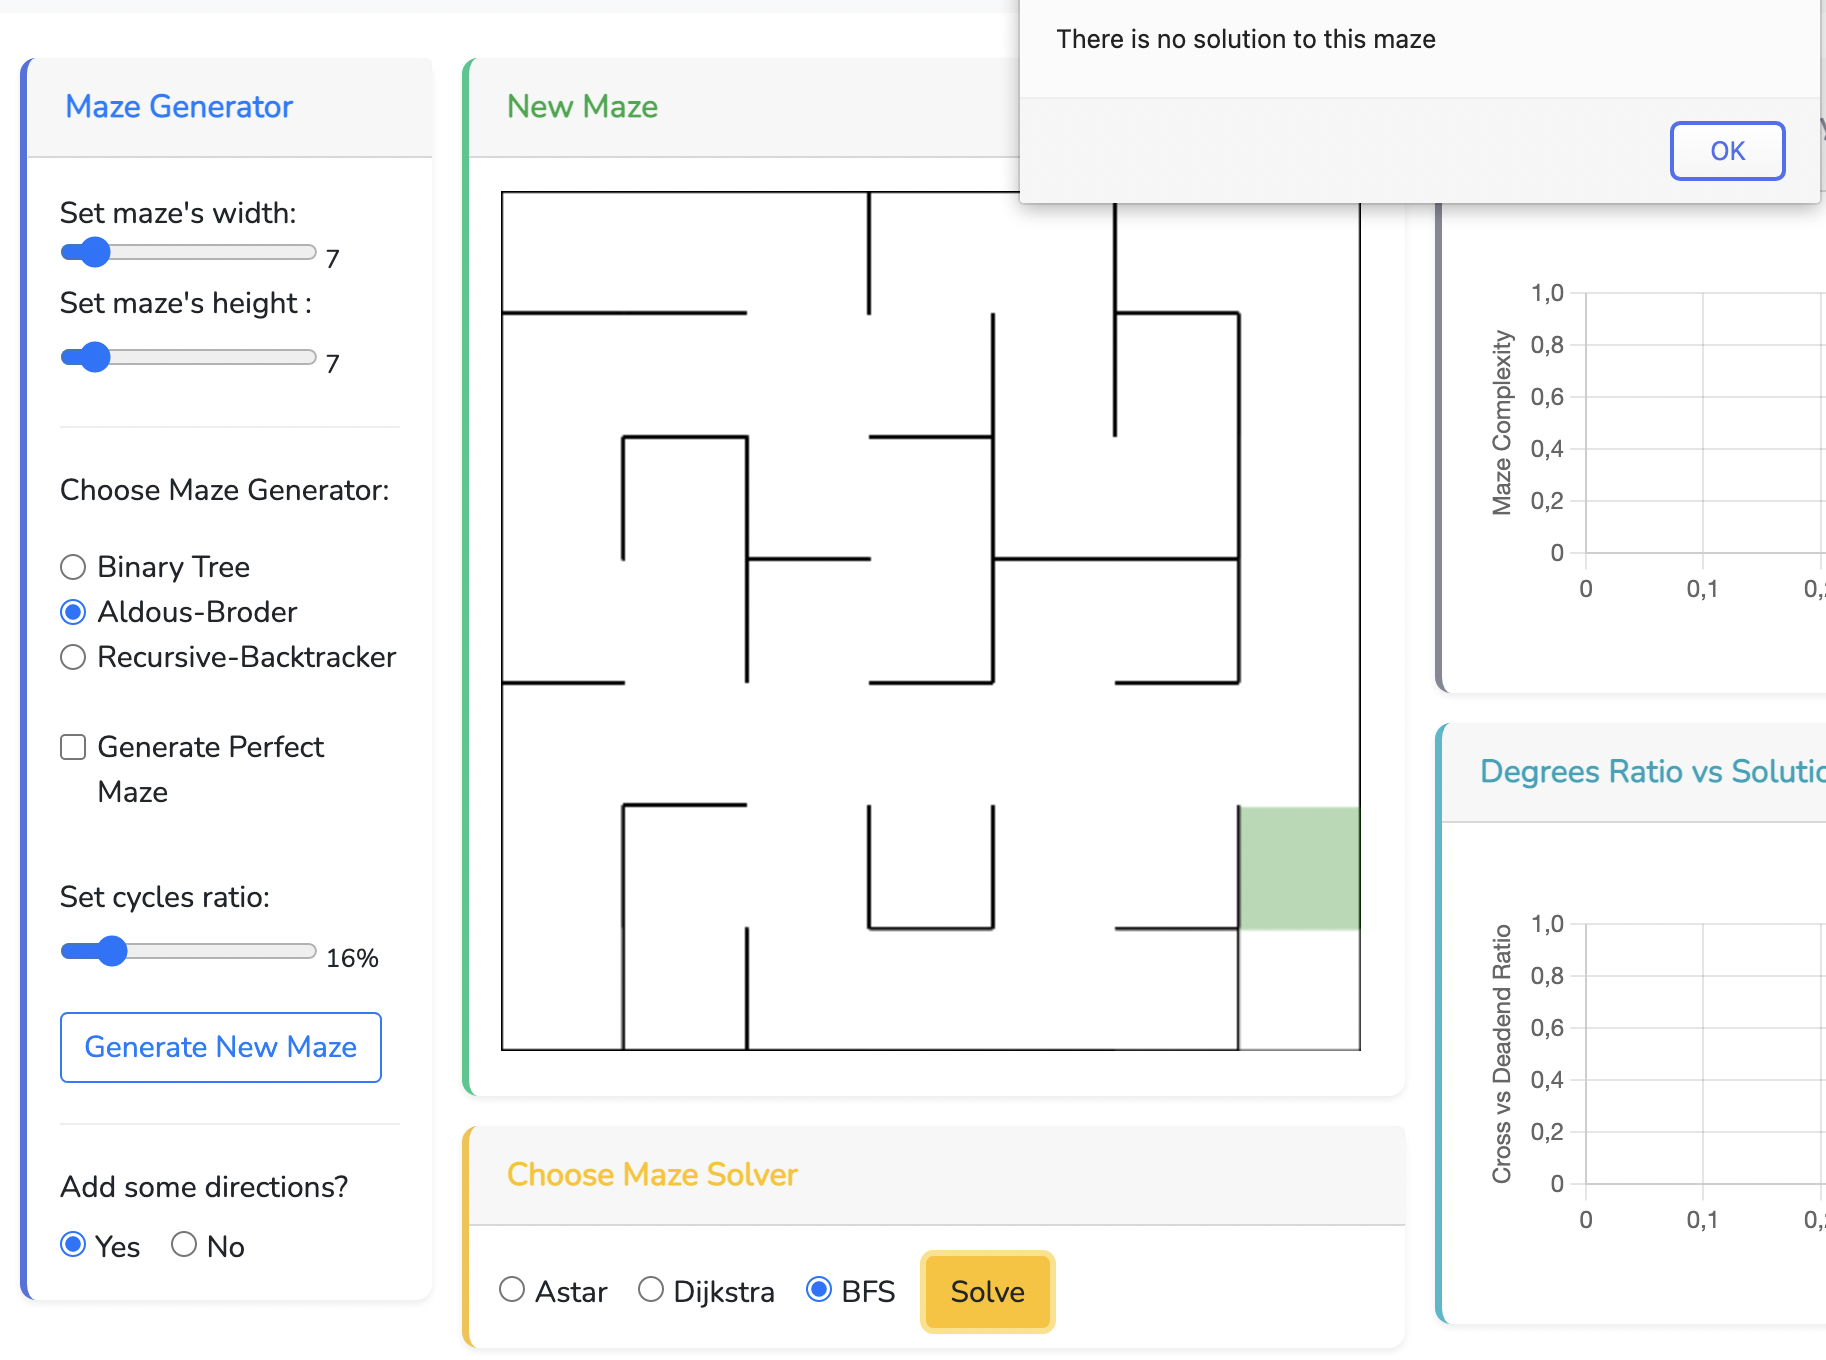
\includegraphics[width=0.5\linewidth]{mazeDirection}
    \caption{Prepared Maze on canvas with a cell chosen to be directed. The maze in the picture can not be solved due to a lack of trespass in the south direction.\\Source: created by the author}
    \end{figure}
\newpage
\textbf{$-$Solver Section}\\
After setting all maze parameters, and populating the maze on canvas, the user can choose out of three implemented maze solvers by selecting the radio button
and clicking on solve button visible in Figure 6.4. One maze can be solved multiple times, by different solvers. Each solution path will be marked in a different colour: 
Astar - blue, BFS - red, Dijkstra - green.\\
\begin{figure}[!h]
    \centering
    \centering
    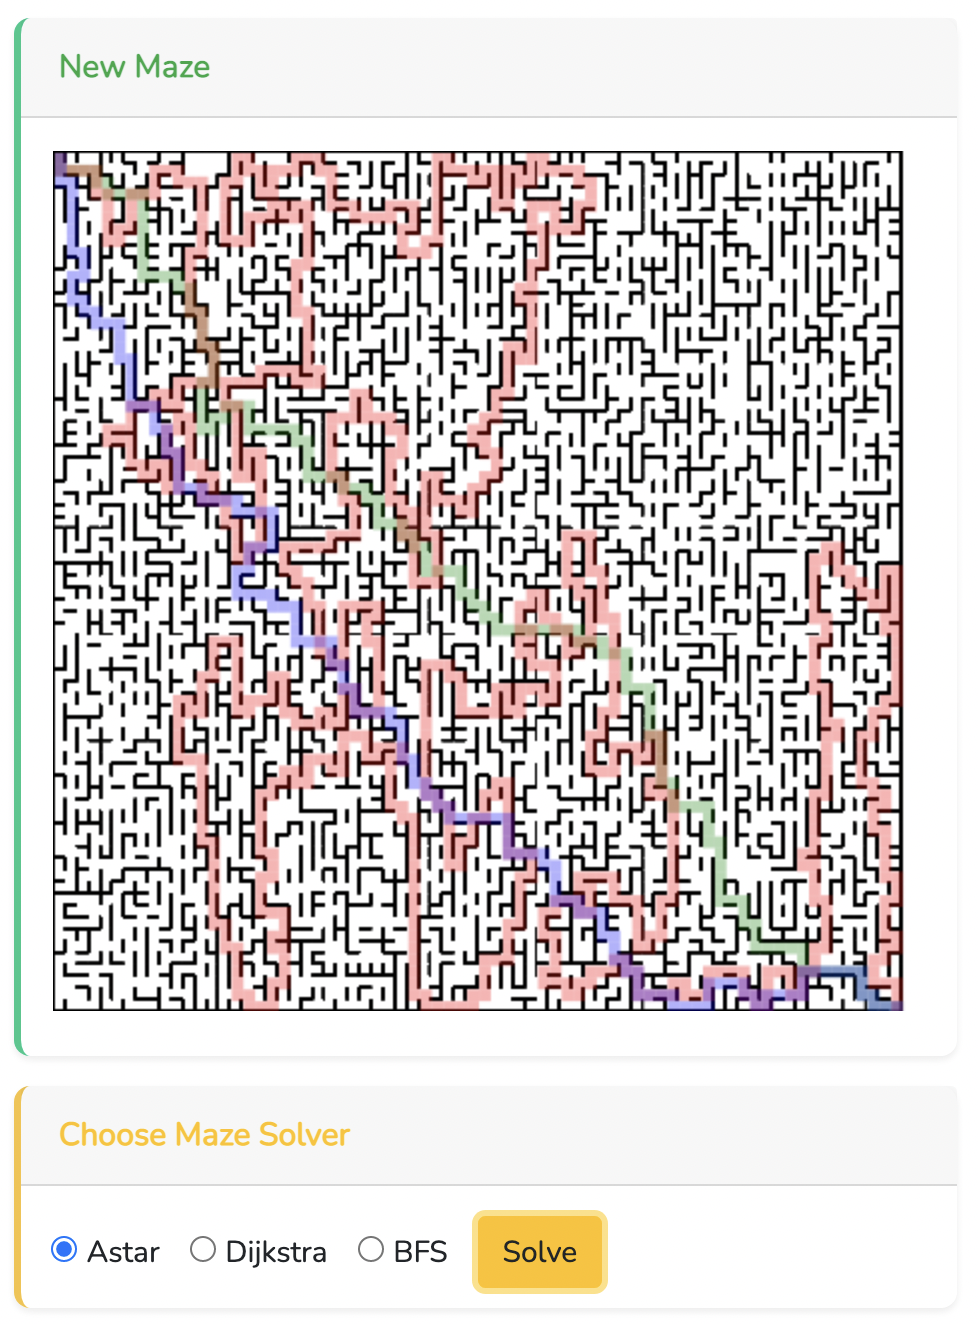
\includegraphics[scale =0.3 ]{mazeSolutions}
    \caption{A maze populated on canvas component, solved by three different solvers.\\Source: created by the author}
    \end{figure}
\newline    
\textbf{$-$Charts Section}\\
Each solution populates a dataset which is drawn into the charts canvas. The chart section contains two separate plots, which collect information about 
generated mazes and their solutions until the Clear All Data button is pressed. The top plot in \textcolor{red}{Figure 6.5 presents a maze complexity versus solution time in milliseconds.
Maze complexity represents a McClendon complexity measure defined in section 4.2.2 by the equation (4.7). Bottom plot in figure 6.5 shows $\frac{cross}{deadend}$
ratio versus solution time in milliseconds. The ratio of dead-ends and crosses is given by the degree distribution given in section 4.1.1 by Definition 23 and the equation (4.1).}\\
\begin{figure}[!h]
    \centering
    \centering
    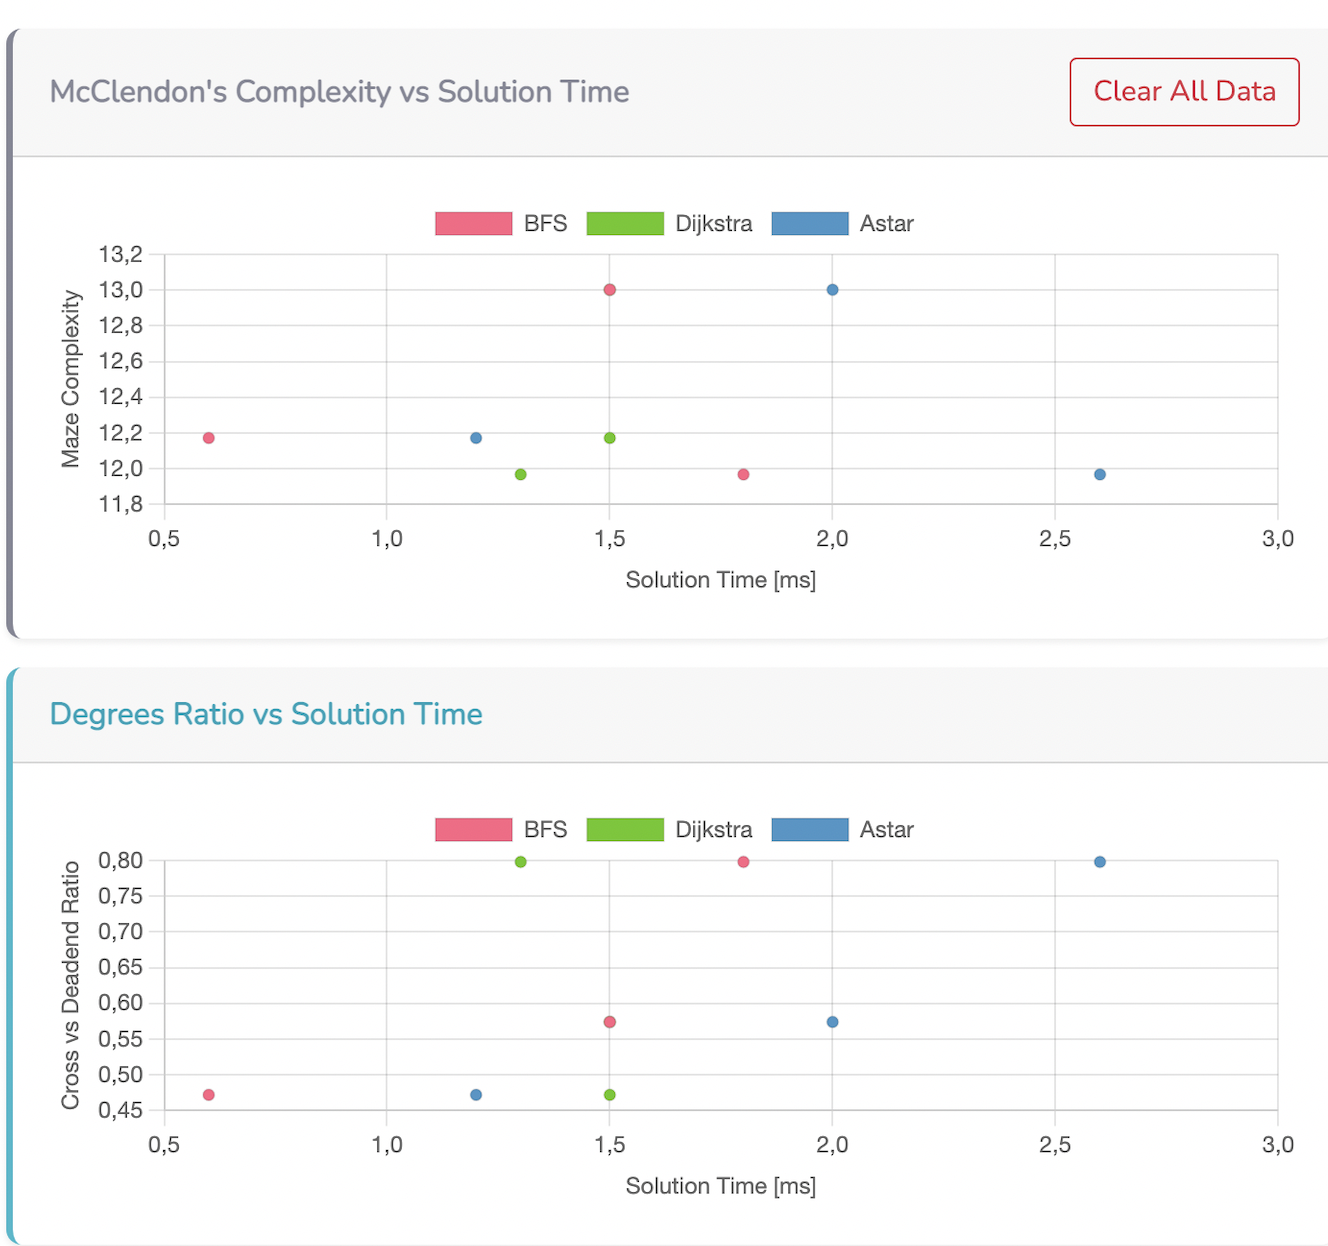
\includegraphics[scale = 0.4]{charts}
    \caption{Plots generated by the data populated by the user using app maze generator and solvers.\\Source: created by the author}
    \end{figure}
\newline    
\textbf{$-$Data Table}\\
In the last table section, all generated data are collected in a data table presented in Figure 6.6. After generating and solving each maze the implemented
functions calculate maze parameters such as average path length defined by Definition 8, degree distribution given by the equation (4.1) in Definition 23,
McClendon's complexity is explained in section 4.2.2 by the equation (4.7), Shannon's entropy is described in section 4.1.2 by the equation (4.3) and time and steps
needed to find a solution for each solver. All data is then inserted into a table. Information about the mazes and their solutions is collected until the Clear
All Data button is pressed.\\
\begin{figure}[!h]
    \centering
    \centering
    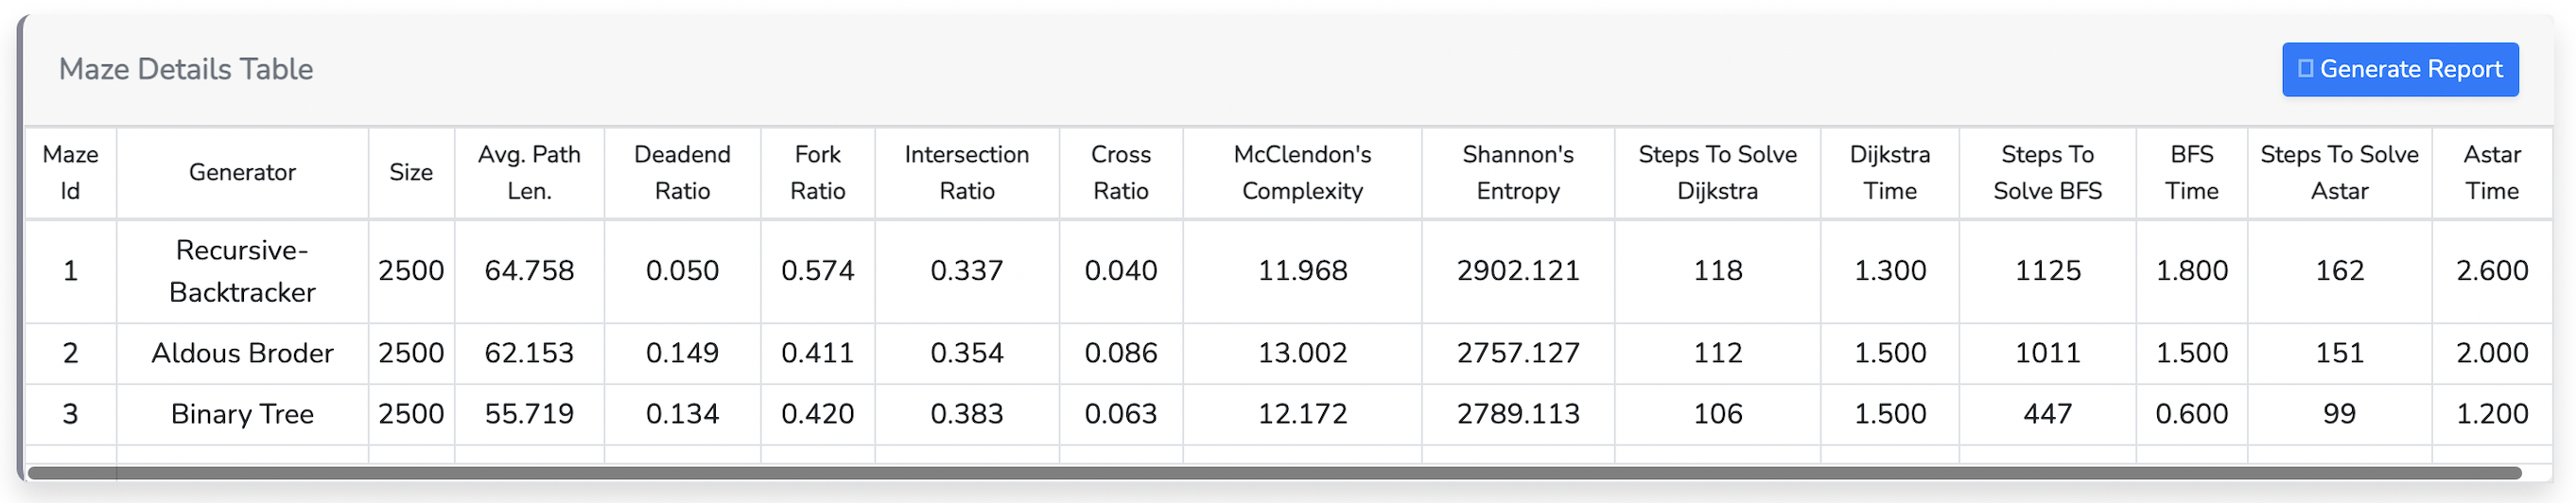
\includegraphics[width = 1 \linewidth]{table}
    \caption{All generated data are stored in the table which may be exported to the PDF file. It gathers all maze and solvers parameters.\\ 
    Source: created by the author }
    \end{figure}
\newline  